\chapter{实数集与函数}
%第一章 实数集与函数

\section{实数}
数学分析研究的基本对象是定义在实数集上的函数.为此,我们先简要叙述实数的有关概念.

\subsection{实数及其性质}

在中学数学课程中,我们知道实数由有理数与无理数两部分组成.\textbf{有理数}可用分数形式 $\frac{p}{q}$($p, q$ 为整数, $q \neq 0$) 表示,也可用有限十进小数或无限十进循环小数来表示;而无限十进不循环小数则称为\textbf{无理数}.有理数和无理数统称为\textbf{实数}.

为了以下讨论的需要,我们把有限小数（包括整数）也表示为无限小数.对此我们 作如下规定 : 对于正有限小数 (包括正整数) $x$, 当 $x=a_{0} . a_{1} a_{2} \cdots a_{n}$ 时, 其中 $0 \leqslant a_{i} \leqslant 9, i=1,2, \cdots, n, a_{n} \neq 0, a_{0}$ 为非负整数, 记
\[
x=a_{0} \cdot a_{1} a_{2} \cdots\left(a_{n}-1\right) 9999 \cdots
\]

而当 $x=a_{0}$ 为正整数时,则记
\[
x=\left(a_{0}-1\right) .9999 \cdots,
\]

例如 $2.001$ 记为 $2.0009999 \cdots$ ;对于负有限小数（包括负整数) $y$, 则先将 $-y$ 表示为无限小数,再在所得无限小数之前加负号,例如 $-8$ 记为 $-7.9999 \cdots ;$ 又规定数 0 表示为 $0.0000 \cdots$ 于是,任何实数都可用一个确定的无限小数来表示.

我们已经熟知比较两个有理数大小的方法.现定义两个实数的大小关系.

\begin{definition}{两个实数的大小关系}{def:两个实数的大小关系}
	给定两个非负实数
	\[
	x=a_{0} . a_{1} a_{2} \cdots a_{n} \cdots, \quad y=b_{0} . b_{1} b_{2} \cdots b_{n} \cdots
	\]

	其中 $a_{0}, b_{0}$ 为非负整数, $a_{k}, b_{k}(k=1,2, \cdots)$ 为整数, $0 \leqslant a_{k} \leqslant 9,0 \leqslant b_{k} \leqslant 9$. 若有
	\[
	a_{k}=b_{k}, k=0,1,2, \cdots,
	\]

	则称 $x$ 与 $y$ 相等,记为 $x=y$;若 $a_{0}>b_{0}$ 或存在非负整数 $l$, 使得
	\[
	a_{k}=b_{k}(k=0,1,2, \cdots, l) \text { 而 } a_{l+1}>b_{l+1}
	\]

	则称 $x$ 大于 $y$ 或 $y$ 小于 $x$, 分别记为 $x>y$ 或 $y<x$.

	对于负实数 $x, y$, 若按上述规定分别有 $-x=-y$ 与 $-x>-y$, 则分别称 $x=y$ 与 $x<y$ ( 或 $y>x$).另外,规定任何非负实数大于任何负实数.
\end{definition}


以下给出通过有限小数来比较两个实数大小的等价条件.为此,先给出如下定义.

\begin{definition}{不足近似与过剩近似}{def:不足近似与过剩近似}
	设 $x=a_{0} . a_{1} a_{2} \cdots a_{n} \cdots$ 为非负实数.称有理数
	\[
	x_{n}=a_{0} . a_{1} a_{2} \cdots a_{n}
	\]

	为实数 $x$ 的 $n$ 位\textbf{不足近似},而有理数
	\[
	\bar{x}_{n}=x_{n}+\frac{1}{10^{n}}
	\]

	称为 $x$ 的 $n$ 位\textbf{过剩近似}, $n=0,1,2, \cdots$.

	对于负实数 $x=-a_{0}, a_{1} a_{2} \cdots a_{n} \cdots$, 其 $n$ 位不足近似与过剩近似分别规定为
	\[
	x_{n}=-a_{0} \cdot a_{1} a_{2} \cdots a_{n}-\frac{1}{10^{n}} \text { 与 } \bar{x}_{n}=-a_{0} \cdot a_{1} a_{2} \cdots a_{n}
	\]
\end{definition}

\begin{remark}
	不难看出,实数 $x$ 的不足近似 $x_{n}$ 当 $n$ 增大时不减, 即有 $x_{0} \leqslant x_{1} \leqslant x_{2} \leqslant \cdots$, 而过剩近似 $\bar{x}_{n}$ 当 $n$ 增大时不增, 即有 $\bar{x}_{0} \geqslant \bar{x}_{1} \geqslant \bar{x}_{2} \geqslant \cdots$.
\end{remark}


我们有以下的命题.

\begin{proposition}{$x>y$ 等价条件}{pro:x>y等价条件}
	设 $x=a_{0} . a_{1} a_{2} \cdots$ 与 $y=b_{0} . b_{1} b_{2} \cdots$ 为两个实数, 则 $x>y$ 的等价条件是:存在非负整数 $n$ , 使得
	\[
	x_{n}>\bar{y}_{n}
	\]

	其中 $x_{n}$ 表示 $x$ 的 $n$ 位不足近似, $\bar{y}_{n}$ 表示 $y$ 的 $n$ 位过剩近似.
\end{proposition}


关于这个命题的证明,以及关于实数的四则运算法则的定义,可参阅本书附录 $\mathrm{I}$第八节.

%例 1
\begin{example}
	设 $x, y$ 为实数, $x<y$. 证明:存在有理数 $r$,满足
	\[
	x<r<y
	\]
\end{example}

\begin{proof}
	由于 $x<y$, 故存在非负整数 $n$, 使得 $\bar{x}_{n}<y_{n}$. 令
	\[
	r=\frac{1}{2}\left(\bar{x}_{n}+y_{n}\right)
	\]

	则 $r$ 为有理数,且有
	\[
	x \leqslant \bar{x}_{n}<r<y_{n} \leqslant y,
	\]

	即得 $x<r<y$.
\end{proof}


为方便起见,通常将全体实数构成的集合记为 $\mathbf{R}$, 即
\[
\mathbf{R}=\{x \mid x \text { 为实数 }\} .
\]

实数有如下一些主要性质:

\begin{enumerate}
	\item 实数集 $\mathbf{R}$ 对加、减、乘、除(除数不为 0 ) 四则运算是封闭的, 即任意两个实数的和、差、积、商(除数不为 0$)$ 仍然是实数.

	\item 实数集是有序的, 即任意两实数 $a, b$ 必满足下述三个关系之一: $a<b, a=b, a>b$.

	\item 实数的大小关系具有传递性, 即若 $a>b, b>c$, 则有 $a>c$.

	\item 实数具有阿基米德(Archimedes)性, 即对任何 $a, b \in \mathbf{R}$, 若 $b>a>0$, 则存在正整数 $n$, 使得 $n a>b$.

	\item 实数集 $\mathbf{R}$ 具有稠密性, 即任何两个不相等的实数之间必有另一个实数,且既有 有理数(见例 1 ), 也有无理数.

	\item 如果在一直线 (通常画成水平直线）上确定一点 $O$ 作为原点, 指定一个方向为正向(通常把指向右方的方向规定为正向), 并规定一个单位长度,则称此直线为\textbf{数轴}. 可以说明: 任一实数都对应数轴上唯一的一点; 反之, 数轴上的每一点也都唯一地代表一个实数. 于是, 实数集 $\mathbf{R}$ 与数轴上的点有着一一对应关系. 在本书以后的叙述中, 常把“实数 $a$ ”与“数轴上的点 $a$ ”这两种说法看作具有相同的含义.
\end{enumerate}

%例 2
\begin{example}
	设 $a, b \in \mathbf{R}$. 证明 : 若对任何正数 $\varepsilon$, 有 $a<b+\varepsilon$, 则 $a \leqslant b$.
\end{example}

\begin{proof}
	用反证法.倘若结论不成立,则根据实数集的有序性,有 $a>b$. 令 $\varepsilon=a-b$, 则 $\varepsilon$ 为正数且 $a=b+\varepsilon$, 但这与假设 $a<b+\varepsilon$ 相矛盾. 从而必有 $a \leqslant b$.
\end{proof}


关于实数的定义与性质的详细论述,有兴趣的读者可参阅本书附录 I.

\subsection{绝对值与不等式}

实数 $a$ 的\textbf{绝对值}定义为
\[
|a|=
\begin{cases}
	a, & a \geqslant 0, \\
	-a, & a<0.
\end{cases}
\]

从数轴上看,数 $a$ 的绝对值 $|a|$ 就是点 $a$ 到原点的距离.

实数的绝对值有如下一些性质：

\begin{enumerate}
	\item $|a|=|-a| \geqslant 0$, 当且仅当 $a=0$ 时有 $|a|=0$.

	\item $-|a| \leqslant a \leqslant|a|$.

	\item $|a|<h \Leftrightarrow -h<a<h,|a| \leqslant h \Leftrightarrow -h \leqslant a \leqslant h(h>0)$.

	\item 对任何 $a, b \in \mathbf{R}$, 都有如下的\textbf{三角形不等式}:
	\[
	|a|-|b| \leqslant|a \pm b| \leqslant|a|+|b|
	\]

	\item $|a b|=|a||b|$.

	\item $\left|\frac{a}{b}\right|=\frac{|a|}{|b|}(b \neq 0)$.
\end{enumerate}


下面只证明性质 4 ,其余性质由读者自行证明.

由性质 2 有
\[
-|a| \leqslant a \leqslant|a|,-|b| \leqslant b \leqslant|b|
\]

两式相加后得到
\[
-(|a|+|b|) \leqslant a+b \leqslant|a|+|b|
\]

根据性质 3 ,上式等价于
\[
|a+b| \leqslant|a|+|b| \tag{1}
\]

将 (1) 式中 $b$ 换成 $-b$, (1) 式右边不变, 即得 $|a-b| \leqslant |a|+|b|$, 这就证明了性质 4 不等式的右半部分.又由 $|a|=|a-b+b|$, 据 (1) 式有
\[
|a| \leqslant|a-b|+|b|
\]

从而得
\[
|a|-|b| \leqslant|a-b| \tag{2}
\]

将 (2) 式中 $b$ 换成 $-b$, 即得 $|a|-|b| \leqslant |a+b|$.性质 4 得证.

\subsection{习题1.1}

1. 设 $a$ 为有理数, $x$ 为无理数.证明:

(1) $a+x$ 是无理数; $\quad(2)$ 当 $a \neq 0$ 时, $a x$ 是无理数.

2. 试在数轴上表示出下列不等式的解:

(1) $x\left(x^{2}-1\right)>0 ; \quad$ (2) $|x-1|<|x-3|$; (3) $\sqrt{x-1}-\sqrt{2 x-1} \geqslant \sqrt{3 x-2}$.

3. 设 $a, b \in \mathbf{R}$. 证明: 若对任何正数 $\varepsilon$, 有 $|a-b|<\varepsilon$, 则 $a=b$.

4. 设 $x \neq 0$, 证明 $\left|x+\frac{1}{x}\right| \geqslant 2$, 并说明其中等号何时成立.

5. 证明 : 对任何 $x \in \mathbf{R}$, 有

(1) $|x-1|+|x-2| \geqslant 1 ; \quad$ (2) $|x-1|+|x-2|+|x-3| \geqslant 2$.

并说明等号何时成立.

6. 设 $a, b, c \in \mathbf{R}^{+}$ ($\mathbf{R}^{+}$ 表示全体正实数的集合).证明
\[
\left|\sqrt{a^{2}+b^{2}}-\sqrt{a^{2}+c^{2}}\right| \leqslant|b-c| .
\]

你能说明此不等式的几何意义吗?

7. 设 $x>0, b>0, a \neq b$. 证明 $\dfrac{a+x}{b+x}$ 介于 1 与 $\dfrac{a}{b}$ 之间.

8. 设 $p$ 为正整数.证明: 若 $p$ 不是完全平方数,则 $\sqrt{p}$ 是无理数.

9. 设 $a, b$ 为给定实数.试用不等式符号(不用绝对值符号)表示下列不等式的解

(1) $|x-a|<|x-b|;$

(2) $|x-a|<x-b ;$

(3) $\left|x^{2}-a\right|<b.$

\section{数集 • 确界原理}

本节中我们先定义 $\mathbf{R}$ 中两类重要的数集——区间与邻域,然后讨论有界集,并给出确界定义和确界原理.

\subsection{区间与邻域}

设 $a, b \in \mathbf{R}$, 且 $a<b.$ 我们称数集 $\{x \mid a<x<b\}$ 为\textbf{开区间}, 记作 $(a, b)$; 数集 $\{x \mid a \leqslant x \leqslant$ $b \mid$ 称为\textbf{闭区间}, 记作 $[a, b] $; 数集 $\{x \mid a \leqslant x<b\}$ 和 $\{x \mid a<x \leqslant b\}$ 都称为\textbf{半开半闭区间}, 分别记作 $[a, b)$ 和 $(a, b].$ 以上这几类区间统称为\textbf{有限区间}. 从数轴上来看, 开区间 $(a, b)$ 表示 $a, b$ 两点间所有点的集合,闭区间 $[a, b]$ 比开区间 $(a, b)$ 多两个端点,半开半闭区间 $[a, b)$ 比开区间 $(a, b)$ 多一个端点 $a$ 等.

满足关系式 $x \geqslant a$ 的全体实数 $x$ 的集合记作 $[a,+\infty)$, 这里符号 $\infty$ 读作“无穷大”, $+\infty$ 读作“正无穷大”.类似地,我们记
\[
(-\infty, a]=\{x \mid x \leqslant a\},(a,+\infty)=\{x \mid x>a\},
\]
\[
(-\infty, a)=\{x \mid x<a\},(-\infty,+\infty)=\{x \mid-\infty<x<+\infty\}=\mathbf{R},
\]
其中 $-\infty$ 读作“负无穷大”. 以上这几类数集都称为\textbf{无限区间}. 有限区间和无限区间统称为\textbf{区间}.

设 $a \in \mathbf{R}, \delta>0 .$ 满足绝对值不等式 $|x-a|<\delta$ 的全体实数 $x$ 的集合称为点 $a$ 的 $\delta$ \textbf{邻域}, 记作 $U(a ; \delta)$, 或简单地写作 $U(a)$, 即有
\[
U(a ; \delta)=\{x|| x-a \mid<\delta\}=(a-\delta, a+\delta)
\]
点 $a$ 的空心 $\delta$ 邻域定义为
\[
\left.U^{\circ}(a ; \delta)=|x| 0<|x-a|<\delta\right\},
\]
它也可简单地记作 $U^{\circ}(a)$. 注意, $U^{\circ}(a ; \delta)$ 与 $U(a ; \delta)$ 的差别在于: $U^{\circ}(a ; \delta)$ 不包含点 $a .$

此外,我们还常用到以下几种邻域:

点 $a$ 的 $\delta$ \textbf{右邻域} $U_{+}(a ; \delta)=[a, a+\delta)$, 简记为 $U_{+}(a)$;

点 $a$ 的 $\delta$ \textbf{左邻域} $U_{-}(a ; \delta)=(a-\delta, a]$, 简记为 $U_{-}(a)$;

($(U_{-}(a)$ 与 $U_{+}(a)$ 去除点 $a$ 后, 分别为点 $a$ 的\textbf{空心} $\delta$ 左、右邻域,简记为 $U^{\circ}(a)$ 与 $U_{+}^{\circ}(a) )$

$\infty$ 邻域 $U(\infty)=|x||x|>M\}$, 其中 $M$ 为充分大的正数(下同）;

$+\infty$ 邻域 $U(+\infty)=\{x \mid x>M\}$;

$-\infty$ 邻域 $U(-\infty)=\{x \mid x<-M\}$.

\subsection{有界集•确界原理}

\begin{definition}{有界与无界}{def:有界与无界}
	设 $S$ 为 $\mathbf{R}$ 中的一个数集.若存在数 $M(L)$, 使得对一切 $x \in S$, 都有 $x \leqslant$ $M(x \geqslant L)$, 则称 $S$ 为\textbf{有上界(下界) 的数集},数 $M(L)$ 称为 $S$ 的一个\textbf{上界(下界)}.

	若数集 $S$ 既有上界又有下界, 则称 $S$ 为\textbf{有界集}. 若 $S$ 不是有界集, 则称 $S$ 为\textbf{无界集}.
\end{definition}

\begin{example}
	证明数集 $\mathbf{N}_{+}=\{n \mid n$ 为正整数 $\}$ 有下界而无上界.
\end{example}

\begin{proof}
	显然,任何一个不大于 1 的实数都是 $\mathbf{N}_{+}$的下界, 故 $\mathbf{N}_{+}$为有下界的数集.

	为证 $\mathbf{N}_{+}$无上界,按照定义只需证明:对于无论多么大的数 $M$, 总存在某个正整数
$n_{0}\left(\in \mathbf{N}_{+}\right)$, 使得 $n_{0}>M$.事实上, 对任何正数 $M$ (无论多么大), 取 $n_{0}=[M]+1$ \footnote{$[x]$ 表示不超过数 $x$ 的最大整数,例如 $[2.9]=2,[-4.1]=-5$.} , 则 $n_{0} \in \mathbf{N}_{+}$, 且 $n_{0}>M .$ 这就证明了 $\mathbf{N}_{+}$无上界.
\end{proof}


读者还可自行证明:任何有限区间都是有界集,无限区间都是无界集;由有限个数 组成的数集是有界集.

若数集 $S$ 有上界,则显然它有无穷多个上界,而其中最小的一个上界常常具有重要的作用,称它为数集 $S$ 的上确界.同样,有下界数集的最大下界,称为该数集的下确界.下面给出数集的上确界和下确界的精确定义.

\begin{definition}{上确界}{def:上确界}
	设 $S$ 是 $\mathbf{R}$ 中的一个数集.若数 $\eta$ 满足:

	(i) 对一切 $x \in S$, 有 $x \leqslant \eta$, 即 $\eta$ 是 $S$ 的上界;

	(ii) 对任何 $\alpha < \eta$, 存在 $x_{0} \in S$, 使得 $x_{0}>\alpha$, 即 $\eta$ 又是 $S$ 的最小上界,

	则称数 $\eta$ 为数集 $S$ 的上确界, 记作
	\[
	\eta=\sup S \footnote{$\sup$ 是拉丁文 supremum (上确界) 一词的简写,下面的 $\mathrm{inf}$ 是拉丁文 infimum (下确界) 一词的简写.}
	\]
\end{definition}

\begin{definition}{下确界}{def:下确界}
	设 $S$ 是 $\mathbf{R}$ 中的一个数集.若数 $\xi$ 满足:

	(i) 对一切 $x \in S$, 有 $x \geqslant \xi$, 即 $\xi$ 是 $S$ 的下界;

	(ii) 对任何 $\beta > \xi$,存在 $x_{0} \in S$, 使得 $x_{0} < \beta$, 即 $\xi$ 又是 $S$ 的最大下界,

	则称数 $\xi$ 为数集 $S$ 的下确界,记作
	\[
	\xi=\inf S
	\]

	上确界与下确界统称为确界.
\end{definition}

\begin{example}
	设 $S=\{x \mid x \text{为区间} (0,1)\text{上的有理数} \}$. 试按上、下确界的定义验证: $\sup S=1, inf S=0$.
\end{example}


\begin{solution}
	先验证 $\sup S=1$ :

	(i) 对一切 $x \in S$, 显然有 $x \leqslant 1$, 即 1 是 $S$ 的上界.

	(ii) 对任何 $\alpha<1$, 若 $\alpha \leqslant 0$, 则任取 $x_{0} \in S$, 都有 $x_{0}>\alpha ;$ 若 $\alpha>0$, 则由有理数集在实数集中的稠密性,在 $(\alpha, 1)$ 上必有有理数 $x_{0}$, 即存在 $x_{0} \in S$, 使得 $x_{0}>\alpha$.

	类似地可验证 $\inf S=0$.
\end{solution}


读者还可自行验证: 闭区间 $[0,1]$ 的上、下确界分别为 1 和 0 ; 对于数集 $E=\left\{\dfrac{(-1)^{n}}{n} \mid n=1,2, \cdots\right\}$, 有 $\sup E=\dfrac{1}{2}, \inf E=-1 ;$ 正整数集 $\mathbf{N}_{+}$有下确界inf $\mathbf{N}_{+}=1$, 而没有上确界.

%注 1
\begin{remark}1由上(下)确界的定义可见,若数集 $S$ 存在上(下)确界,则一定是唯一的.又若数集 $S$ 存在上、下确界, 则有 $\inf S \leqslant \sup S$.
\end{remark}


%注 2
\begin{remark}2从上面一些例子可见,数集 $S$ 的确界可能属于 $S$,也可能不属于 $S$.
\end{remark}

\begin{example}
	设数集 $S$ 有上确界.证明
	\[
	\eta=\sup S \in S \Leftrightarrow \eta=\max S \footnote{记号 $\max$ 是 maximum (最大) 一词的简写, $\eta=\max S$ 表示数 $\eta$ 是数集 $S$ 中最大的数.以下将出 现的记号 $\min$ 是 minimum (最小) 一词的简写, $\min S$ 表示数集 $S$ 中最小的数. }
	\]
\end{example}

\begin{proof}
	$\Rightarrow$ ) 设 $\eta=\sup S \in S$, 则对一切 $x \in S$, 有 $x \leqslant \eta$, 而 $\eta \in S$, 故 $\eta$ 是数集 $S$ 中最大的数, 即 $\eta=\max S$.

	$\Leftarrow$ ) 设 $\eta=\max S$, 则 $\eta \in S ;$ 下面验证 $\eta=\sup S$ :

	(i) 对一切 $x \in S$, 有 $x \leqslant \eta$, 即 $\eta$ 是 $S$ 的上界;

	(ii) 对任何 $\alpha<\eta$, 只需取 $x_{0}=\eta \in S$, 则 $x_{0}>\alpha$.从而满足 $\eta=\sup S$ 的定义.
\end{proof}


关于数集确界的存在性,我们给出如下确界原理.

\begin{theorem}{确界原理}{the:确界原理}
	设 $S$ 为非空数集.若 $S$ 有上界,则 $S$ 必有上确界;若 $S$ 有下界,则 $S$ 必有下确界.
\end{theorem}

\begin{proof}
	我们只证明关于上确界的结论,后一结论可类似地证明.

	为叙述方便,不妨设 $S$ 含有非负数.由于 $S$ 有上界, 故可找到非负整数 $n$,使得

	1) 对于任何 $x \in S$, 有 $x<n+1$ ；

	2) 存在 $a_{0} \in S$,使 $a_{0} \geqslant n$.

	对半开区间 $[n, n+1)$ 作 10 等分, 分点为 $n .1, n .2, \cdots, n .9$, 则存在 $0,1,2, \cdots, 9$ 中的一个数 $n_{1}$, 使得

	1) 对于任何 $x \in S$, 有 $x<n.n_1+\frac{1子}{10}$ ；

	2) 存在 $a_{1} \in S$,使 $a_{1} \geqslant n . n_{1}$.

	再对半开区间 $\left[n.n_{1}, n . n_{1}+\frac{1}{10}\right) $  作  10  等分, 则存在 $ 0,1,2, \cdots, 9 $ 中的一个数 $ n_{2}, $ 使得

	1) 对于任何 $x \in S$, 有 $x<n \cdot n_{1} n_{2}+\frac{1}{10^{2}}$;

	2) 存在 $a_{2} \in S$, 使 $a_{2} \geqslant n.n_{1} n_{2}$.

	继续不断地 10 等分在前一步骙中所得到的半开区间, 可知对任何 $k=1,2, \cdots$, 存在 $0,1,2, \cdots, 9$ 中的一个数 $n_{k}$, 使得

	1) 对于任何 $ x \in S $, 有 \[ x<n.n_{1} n_{2} \cdots n_{k}+\frac{1}{10^{k}} ;\tag{1}\]

	2) 存在 $a_{k} \in S$, 使 $a_{k} \geqslant n . n_{1} n_{2} \cdots n_{k}$.

	将上述步骤无限地进行下去,得到实数 $\eta=n.n_{1} n_{2} \cdots n_{k} \cdots .$ 以下证明 $\eta=\sup S$. 为此只需证明:

	(i) 对一切 $x \in S$, 有 $x \leqslant \eta ;$ (ii) 对任何 $\alpha<\eta$, 存在 $a^{\prime} \in S$, 使 $\alpha<a^{\prime}$.

	倘若结论 (i) 不成立, 即存在 $x \in S$,使 $x>\eta$, 则可找到 $x$ 的 $k$ 位不足近似 $x_{k}$, 使
	\[
	x_{k}>\bar{\eta}_{k}=n.n_{1} n_{2} \cdots n_{k}+\frac{1}{10^{k}}
	\]

	从而得
	\[
	x>n.n_{1} n_{2} \cdots n_{k}+\frac{1}{10^{k}},
	\]

	但这与不等式(1) 相矛盾.于是 (i) 得证.

	现设 $\alpha<\eta$, 则存在 $k$,使 $\eta$ 的 $k$ 位不足近似 $\eta_{k}>\bar{\alpha}_{k}$, 即
	\[
	n.n_{1} n_{2} \cdots n_{k}>\bar{\alpha}_{k}
	\]

	根据数 $\eta$ 的构造,存在 $a^{\prime} \in S$, 使 $a^{\prime} \geqslant \eta_{k}$, 从而有
	\[
	a^{\prime} \geqslant \eta_{k}>\bar{\alpha}_{k} \geqslant \alpha,
	\]

	即得到 $\alpha<a^{\prime}$. 这说明 (ii) 成立.
\end{proof}


在本书中确界原理是极限理论的基础,读者应给予充分的重视.

\begin{example}
	设 $A, B$ 为非空数集,满足:对一切 $x \in A$ 和 $y \in B$ 有 $x \leqslant y .$ 证明:数集 $A$ 有上确 界,数集 $B$ 有下确界, 且
	\[
	\sup A \leqslant \inf B. \tag{2}
	\]
\end{example}

\begin{proof}
	由假设,数集 $B$ 中任一数 $y$ 都是数集 $A$ 的上界, $A$ 中任一数 $x$ 都是 $B$ 的下界, 故由确界原理推知数集 $A$ 有上确界,数集 $B$ 有下确界.

	现证不等式 ( 2 ). 对任何 $y \in B, y$ 是数集 $A$ 的一个上界,而由上确界的定义知, $\sup A$ 是数集 $A$ 的最小上界, 故有 $\sup A \leqslant y$. 而此式又表明数 $\sup A$ 是数集 $B$ 的一个下
界, 故由下确界定义证得 $\sup A \leqslant \inf B$.
\end{proof}


\begin{example}
	设 $A, B$ 为非空有界数集, $S=A \cup B$. 证明:

	(i) $\sup S=\max \{\sup A, \sup B\}$;

	(ii) $\inf S=\min \{\inf A, \inf B\}$.
\end{example}

\begin{proof}
	由于 $S=A \cup B$, 显然 $S$ 也是非空有界数集,因此 $S$ 的上、下确界都存在.

	(i) 对任 何 $x \in S$, 有 $x \in A$ 或 $x \in B \Rightarrow x \leqslant \sup A$ 或 $x \leqslant \sup B$, 从而 有 $x \leqslant$ $\max \{\sup A, \sup B\}$, 故得 $\sup S \leqslant \max \{\sup A, \sup B\} .$ 另一方面, 对任何 $x \in A$, 有 $x \in S \Rightarrow x \leqslant \sup S \Rightarrow \sup A \leqslant \sup S ;$ 同理又有 $\sup B \leqslant \sup S.$ 所以 $\sup S \geqslant \max \{\sup A, \sup B\}$.

	综上, 即证得 $\sup S=\max \{\sup A, \sup B \mid$.

	(ii) 可类似地证明.
\end{proof}


若把 $+\infty$ 和 $-\infty$ 补充到实数集中,并规定任一实数 $a$ 与 $+\infty,-\infty$ 的大小关系为: $a<+\infty, a>-\infty,-\infty<+\infty$, 则确界概念可扩充为 : 若数集 $S$ 无上界, 则定义 $+\infty$ 为 $S$ 的\textbf{非正常上确界}, 记作 $\sup S=+\infty$; 若 $S$ 无下界, 则定义 $-\infty$ 为 $S$ 的\textbf{非正常下确界},记作 $\inf S=-\infty$ 相应地,前面定义 2 和定义 3 中所定义的确界分别称为\textbf{正常上、下确界}.

在上述扩充意义下,我们有

\textbf{推广的确界原理} $\quad$ 任一非空数集必有上、下确界(正常的或非正常的).

例如,对于正整数集 $\mathbf{N}_{+}$, 有 $\inf \mathbf{N}_{+}=1, \sup \mathbf{N}_{+}=+\infty ;$ 对于数集
\[
S=\left\{y \mid y=2-x^{2}, x \in \mathbf{R}\right\} , \tag{3}
\]

有 $\inf S=-\infty$, $\sup S=2$.

\subsection{习题1.2}

1. 用区间表示下列不等式的解

(1) $|1-x|-x \geqslant 0;$

(2) $\left|x+\frac{1}{x}\right| \leqslant 6 ;$

(3) $(x-a)(x-b)(x-c)>0$ ($a, b, c$ 为常数, 且 $a<b<c$) ;

(4) $\sin x \geqslant \frac{\sqrt{2}}{2}$.

2. 设 $S$ 为非空数集.试对下列概念给出定义:

(1) $S$ 无上界；

(2) $S$ 无界.

3. 试证明由 $(3)$ 式所确定的数集 $S$ 有上界而无下界.

4. 求下列数集的上、下确界, 并依定义加以验证:

(1) $S=\left\{x \mid x^{2}<2\right\};$

(2) $S=\left\{x \mid x=n !, n \in \mathbf{N}_{+}\right\};$

(3) $S=\{x \mid x$ 为 $(0,1)$ 上的无理数;

(4) $S=\left\{x \mid x=1-\frac{1}{2^{n}}, n \in \mathbf{N},\right\} .$

5. 设 $S$ 为非空有下界数集.证明:
$\inf S=\xi \in S \Leftrightarrow \xi=\min S$

6. 设 $S$ 为非空数集,定义 $S^{-}=\{x \mid -x \in S\} .$ 证明：

(1) inf $S=-\sup S ;$

(2) sup $S^{-}=-\inf S$

7. 设 $A, B$ 皆为非空有界数集,定义数集
\[A+B=\{z \mid z=x+y, x \in A, y \in B\}\]

证明: $(1) \sup (A+B)=\sup A+\sup B;$

$(2) \inf (A+B)=\inf A+\inf B$

\section{函数概念}

关于函数概念,在中学数学中我们已有了初步的了解,本节将对此作进一步的讨论.

\subsection{函数的定义}
\begin{definition}{函数}{def:函数}
	给定两个实数集 $D$ 和 $M$, 若有对应法则 $f$, 使对每一个 $x \in D$, 都有唯一的 $y \in M$ 与它相对应,则称 $f$ 是定义在数集 $D$ 上的函数, 记作
	\[
	\begin{aligned}
		f: & D \rightarrow M \\
		& x \mapsto y
	\end{aligned}\tag{1}
	\]

	数集 $D$ 称为函数 $f$ 的\textbf{定义域}, $x$ 所对应的 $y$ 称为 $f$ 在点 $x$ 的\textbf{函数值},常记为 $f(x)$.全体函数值的集合
	\[
	f(D)=\{y \mid y=f(x), x \in D\}(\subset M)
	\]

	称为函数 $f$ 的\textbf{值域}.

	(1) 中第一式 “ $f: D \rightarrow M$ ” 表示按法则 $f$ 建立数集 $D$ 到 $M$ 的函数关系； 第二式 “ $x \mapsto y$ ” 表示这两个数集中元素之间的对应关系,也可记为“ $x \mapsto f(x)$ ” 习惯上,我们称此函数关系中的 $x$ 为\textbf{自变量}, $y$ 为\textbf{因变量}.
\end{definition}


关于函数的定义,我们作如下几点说明：

1. 定义 1 中的实数集 $M$ 常以 $\mathbf{R}$ 来代替,于是定义域 $D$ 和对应法则 $f$ 就成为确定函数的两个主要因素.所以,我们也常用
\[
y=f(x), x \in D
\]
表示一个函数.由此,我们说某两个函数相同, 是指它们有相同的定义域和对应法则.如果两个函数对应法则相同而定义域不同,那么这两个函数仍是不相同的.例如 $f(x)=1, x \in \mathbf{R}$ 和 $g(x)=1, x \in \mathbf{R} \backslash\{0\}$ 是不相同的两个函数.另一方面,两个相同的函数, 其对应法则的表达形式可能不同,例如
\[
\varphi(x)=|x|, x \in \mathbf{R} \text { 和 } \psi(x)=\sqrt{x^{2}}, x \in \mathbf{R}
\]

2. 我们在中学数学中已经知道,表示函数的主要方法是解析法(公式法),即用数学运算式子来表示函数.这时,函数的定义域常取使该运算式子有意义的自变量值的全体,通常称为存在域.在这种情况下,函数的定义域(即存在域) $D$ 可省略不写,而只用对应法则 $f$ 来表示一个函数,此时可简单地说“函数 $y=f(x) $” 或“函数 $f$”.

3. 函数 $f$ 给出了 $x$ 轴上的点集 $D$ 到 $y$ 轴上点集 $M$ 之间的单值对应,也称为映射. 对于 $a \in D, f(a)$ 称为映射 $f$ 下 $a$ 的象, $a$ 则称为 $f(a)$ 的原象.

4. 在函数定义中,对每一个 $x \in D$, 只能有唯一的一个 $y$ 值与它对应, 这样定义的函数称为单值函数. 若同一个 $x$ 值可以对应多于一个的 $y$ 值,则称这种函数为多值函数. 在本书范围内, 我们只讨论单值函数.

\subsection{函数的表示法}

在中学课程里, 我们已经知道函数的表示法主要有三种, 即解析法(或称公式法)、 列表法和图像法.

有些函数在其定义域的不同部分用不同的公式表达,这类函数通常称为分段函 数.例如,函数
\[
\operatorname{sgn} x=
\begin{cases}
	1, & x>0, \\
	0, & x=0, \\
	-1, & x<0
\end{cases}
\]
是分段函数,称为符号函数,其图像如图 $1-1$ 所示.又如函数 $f(x)=|x|$ 也可用如下的分段函数形式来表示：
\[
f(x)=\left\{\begin{array}{l}
	x, \quad x \geqslant 0 \\
	-x, x<0
\end{array}\right.
\]

它还可表示为 $f(x)=x \operatorname{sgn} x$.


\begin{figure}
	\centering
	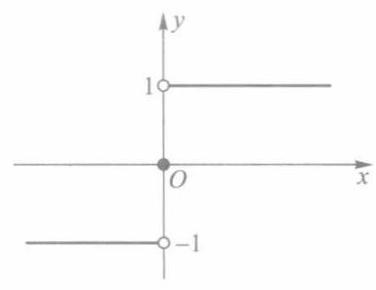
\includegraphics[width=.3\textwidth]{images/P001}
	\caption{图 $1-1$}
	\label{fig:P001}
\end{figure}


函数 $ y=f(x), x \in D $ 又可用有序数对的集合
\[G=\{(x, y) \mid y=f(x), x \in D\}\]
来表示.在坐标平面上,集合 $G$ 的每一个元素 $(x, y)$ 表示平面上的一个点,因而集合 $G$ 在坐标平面上描绘出这个函数的图像.这就是用图像法表示函数的依据.

有些函数只能用语言来描述,如定义在 $\mathbf{R}$ 上的狄利克雷(Dirichlet) 函数
\[
D(x)=
\begin{cases}
	1, & \text { 当 } x \text { 为有理数, } \\
	0, & \text { 当 } x \text { 为无理数 }
\end{cases}
\]
和定义在 $[0,1]$ 上的黎曼 (Riemann) 函数
\[
R(x)=\left\{\begin{array}{l}
	\frac{1}{q}, \quad \text { 当 } x=\frac{p}{q}\left(p, q \in \mathbf{N}_{+}, \frac{p}{q}\right. \text { 为既约真分数), } \\
	0, \quad \text { 当 } x=0,1 \text { 和 }(0,1) \text { 内的无理数. }
\end{array}\right.
\]

图 $1-2$ 和图 $1-3$ 分别是这两个函数的示意图.


\begin{figure}
	\centering
	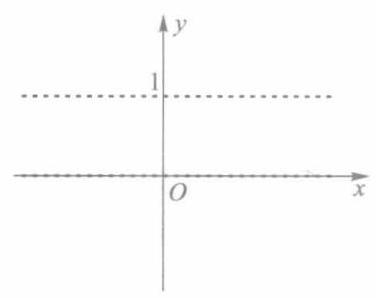
\includegraphics[width=.3\textwidth]{images/P002}
	\caption{图 $1-2$}
	\label{fig:P002}
\end{figure}


\begin{figure}
	\centering
	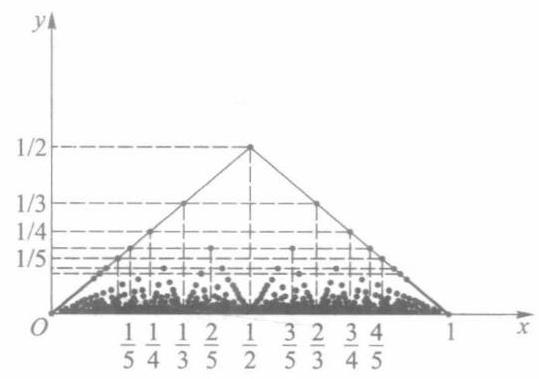
\includegraphics[width=.3\textwidth]{images/P003}
	\caption{图 $1-3$}
	\label{fig:P003}
\end{figure}

\subsection{函数的四则运算}

给定两个函数 $ f, x \in D_{1} $ 和 $ g, x \in D_{2} .$ 记 $ D=D_{1} \cap D_{2} $, 并设 $ D \neq \varnothing .$ 我们定义 $ f $ 与 $ g $ 在 $D$ 上的和、差、积运算如下:
\[
\begin{aligned}
	&F(x)=f(x)+g(x), x \in D, \\
	&G(x)=f(x)-g(x), x \in D, \\
	&H(x)=f(x) g(x), x \in D .
\end{aligned}
\]
若在 $D$ 中剔除使 $g(x)=0$ 的 $x$ 值, 即令
\[
D^{*}=D_{1} \cap\left\{x \mid g(x) \neq 0, x \in D_{2}\right\} \neq \varnothing
\]
可在 $D^{*}$ 上定义 $f$ 与 $g$ 的商的运算如下：
\[
L(x)=\frac{f(x)}{g(x)}, x \in D^{*}
\]

%注
\begin{remark}
若 $D=D_{1} \cap D_{2}=\varnothing$, 则 $f$ 与 $g$ 不能进行四则运算.例如,设
\[
\begin{aligned}
    &f(x)=\sqrt{1-x^{2}}, x \in D_{1}=\{x|| x \mid \leqslant 1\} \\
    &g(x)=\sqrt{x^{2}-4}, x \in D_{2}=\{x|| x \mid \geqslant 2\}
\end{aligned}
\]

由于 $D_{1} \cap D_{2}=\varnothing $, 所以表达式
\[
f(x)+g(x)=\sqrt{1-x^{2}}+\sqrt{x^{2}-4}
\]
是没有意义的.

以后为叙述方便, 函数 $f$ 与 $g$ 的和、差、积、商常分别写作
\[
f+g, f-g, f g, \frac{f}{g}
\]
\end{remark}


\subsection{复合函数}

设有两函数
\[
\begin{aligned}
	&y=f(u), u \in D \\
	&u=g(x), x \in E
\end{aligned}\tag{2}
\]

记 $E^{*}=\{x \mid g(x) \in D\} \cap E .$ 若 $E^{*} \neq \varnothing $, 则对每一个 $x \in E^{*}$, 可通过函数 $g$ 对应 $D$ 上唯 一的一个值 $u$, 而 $u$ 又通过函数 $f$ 对应唯一的一个值 $y$. 这就确定了一个定义在 $E^{*}$ 上的 函数, 它以 $x$ 为自变量, $y$ 为因变量,记作
\[
y=f(g(x)), x \in E^{*} \text { 或 } y=(f \circ g)(x), x \in E^{*} ,
\]
称为函数 $f$ 和 $g$ 的\textbf{复合函数}.并称 $f$ 为\textbf{外函数}, $g$ 为\textbf{内函数}, (2) 式中的 $u$ 为中间变量. 函数 $f$ 和 $g$ 的复合运算也可简单地写作 $f \circ g$.

%例
\begin{example}
$\mathbf{1}$ 函数 $y=f(u)=\sqrt{u}, u \in D=[0,+\infty)$ 与 函数 $u=g(x)=1-x^{2}, x \in E=\mathbf{R}$ 的复合 函数为
\[
y=f(g(x))=\sqrt{1-x^{2}} \quad \text { 或 } \quad(f \circ g)(x)=\sqrt{1-x^{2}},
\]
其定义域 $E^{*}=[-1,1] \subset E$.
\end{example}


复合函数也可由多个函数相继复合而成.例如,由三个函数 $y=\sin u, u=\sqrt{v}$ 与 $v=1$ $x^{2}$ (它们的定义域取为各自的存在域)相继复合而得的复合函数为
\[
y=\sin \sqrt{1-x^{2}}, x \in[-1,1]
\]

%注
\begin{remark}
当且仅当 $E^{*} \neq \varnothing$ (即 $\left.D \cap g(E) \neq \varnothing\right)$ 时, 函数 $f$ 与 $g$ 才能进行复合.例如,以 $y=f(u)=\arcsin u, u \in D=[-1,1]$ 为外函数, $u=g(x)=2+x^{2}, x \in E=\mathbf{R}$ 为内函数, 就不能进行复合.这是因为外函数的定义域 $D=[-1,1]$ 与内函数的值域 $g(E)=[2,+\infty)$ 不相交.
\end{remark}


\subsection{反函数}

函数 $y=f(x)$ 的自变量 $x$ 与因变量 $y$ 的关系往往是相对的. 有时我们不仅要研究 $y$ 随 $x$ 而变化的状况, 也要研究 $x$ 随 $y$ 而变化的状况. 对此, 我们引人反函数概念.

设函数
\[
y=f(x), x \in D \tag{3}
\]
满足 : 对于值域 $f(D)$ 上的每一个 $y, D$ 中有且只有一个 $x$, 使得
\[
f(x)=y
\]
则按此对应法则得到一个定义在 $f(D)$ 上的函数,称这个函数为 $f$ 的反函数,记作
\[
\begin{gathered}
	f^{-1}: f(D) \rightarrow D, \\
	\quad y \mapsto x
\end{gathered}
\]
或
\[
x=f^{-1}(y), y \in f(D) \tag{4}
\]

\begin{remark}
	1 函数 $f$ 有反函数,意味着 $f$ 是 $D$ 与 $f(D)$ 之间的一个一一映射.我们称 $f^{-1}$ 为映射 $f$ 的\textbf{逆映射},它把集合 $f(D)$ 映射到集合 $D$, 即把 $f(D)$ 中的每一个值 $f(a)$ 对应到 $D$ 上唯 一的一个值 $a$.这时称 $a$ 为逆映射 $f^{-1} 下 f(a)$ 的象,而 $f(a)$ 则是 $a$ 在逆映射 $f^{-1} 下$ 的原象.

	从上述讨论还可看到, 函数 $f$ 也是函数 $f^{-1}$ 的反函数.或者说, $f$ 与 $f^{-1}$ 互为反函数. 并有
	\[
	\begin{gathered}
		f^{-1}(f(x)) \equiv x, x \in D \\
		f\left(f^{-1}(y)\right) \equiv y, y \in f(D)
	\end{gathered}
	\]
\end{remark}

\begin{remark}
	2 在反函数 $f^{-1}$ 的表示式(4)中, 是以 $y$ 为自变量, $x$ 为因变量.若按习惯,仍用 $x$ 作为自变量的记号, $y$ 作为因变量的记号,则函数 (3) 的反函数 (4) 可改写为
	\[
	y=f^{-1}(x), x \in f(D) \tag{5}
	\]
例如,按习惯记法, 函数 $y=a x+b(a \neq 0), y=a^{x}(a>0, a \neq 1)$ 与 $y=\sin x, x \in\left[-\frac{\pi}{2}, \frac{\pi}{2}\right]$ 的反函数分别是
	\[
	y=\frac{x-b}{a}, y=\log _{a} x \text { 与 } y=\arcsin x \text {. }
	\]
\end{remark}


应该注意,尽管反函数 $f^{-1}$ 的表示式(4)与(5)的形式不同,但它们仍表示同一个函数, 因为它们的定义域都是 $f(D)$, 对应法则都是 $f^{-1}$, 只是所用变量的记号不同而已.

\begin{example}
	设 $a>0, n(\geqslant 2)$ 是自然数.证明: 方程 $x^{n}=a$ 有唯一的正数解.这个解称为 $a$ 的 $n$ 次正根(即算术根), 记为 $\sqrt[n]{a}$ 或者 $a^{\frac{1}{n}}$.
\end{example}

\begin{proof}
	为简单起见,我们仅证 $n=2$ 的情形.

	首先证明存在性. $a=1$ 时显然有解. 又由于方程
	\[
	x^{2}=a
	\]

	与方程
	\[
	\frac{1}{x^{2}}=\frac{1}{a}
	\]

	同解,所以仅需考虑 $0<a<1$ 的情形.设
	\[
	E=\left\{x \mid x>0, x^{2}<a\right\}
	\]

	因为 $a \in E$, 且 1 是 $E$ 的一个上界, 所以由确界定理, $E$ 的上确界存在,记为 $c=\sup E$. 由确界定义易得 $a \leqslant c \leqslant 1$.下面证明 $c^{2}=a$.

	(1) 若 $c^{2}>a$,根据实数的阿基米德性质,存在自然数 $m$, 使得 $\frac{1}{m}<\frac{c^{2}-a}{2}, \frac{1}{m}<c$. 由确界的定义,存在 $x_{0} \in E, x_{0}>c-\frac{1}{m}>0$, 从而
	\[
	x_{0}^{2}>\left(c-\frac{1}{m}\right)^{2}=c^{2}-2 \cdot \frac{c}{m}+\frac{1}{m^{2}}>c^{2}-\frac{2}{m}>c^{2}-\left(c^{2}-a\right)=a
	\]

	这与 $x_{0} \in E$ 矛盾, 说明 $c^{2} \leqslant a$.

	(2) 同理可证 $c^{2}<a$ 也不成立.由此得到 $c^{2}=a$.

	再证明唯一性.对任意正数 $b(\neq c), b^{2}-a=b^{2}-c^{2}=(b-c)(b+c) \neq 0$, 这证明了解的唯一性.
\end{proof}


设 $a>0, m, n, p$ 为正整数,规定 $a^{\frac{m}{n}}=\left(a^{\frac{1}{n}}\right)^{m}$, 那么有 $a^{\frac{p m}{p n}}=\left(a^{\frac{1}{n n}}\right)^{p m}=a^{\frac{m}{n}}$. 我们将此性质的证明留作匀题.

\subsection{初等函数}

在中学数学中,读者已经熟悉基本初等函数有以下六类：

常量函数 $y=c \quad(c$ 是常数 $) ;$

幂函数 $y=x^{\alpha}(\alpha$ 为实数 $)$;

指数函数 $\quad y=a^{x}(a>0, a \neq 1)$;

对数函数 $\quad y=\log _{a} x(a>0, a \neq 1) ;$

三角函数 $y=\sin x$ (正弦函数), $y=\cos x$( 余弦函数 ), $y=\tan x$ (正切函数 $), y=\cot x$ (余切函数);

反三角函数 $y=\arcsin x$ (反正弦函数) , $y=\arccos x$( 反余弦函数), $y=\arctan x$( 反正切函数 ), $y=\operatorname{arccot} x$( 反余切函数 ).

这里我们要指出, 幂函数 $y=x^{\alpha}$ 和指数函数 $y=a^{x}$ 都涉及乘幂,而在中学数学课程中只给出了有理指数乘幂的定义. 下面我们借助确界来定义无理指数幂,使它与有理指数幂一起构成实指数乘幂, 并保持有理指数幂的基本性质.

\begin{definition}{实指数乘幂}{def:实指数乘幂}
	给定实数 $a>0, a \neq 1$. 设 $x$ 为无理数,我们规定
	\[
	a^{x}=\left\{\begin{array}{l}
		\sup _{r<x}\left\{a^{r} \mid r \text { 为有理数 }\right\} \text {, 当 } a>1 \text { 时, }\quad (6) \\
		\inf _{r<x}\left\{a^{r} \mid r \text { 为有理数 }\right\}, \text { 当 } 0<a<1 \text { 时. }\quad (7)
	\end{array}\right.
	\]
\end{definition}

\begin{remark}
	1 对任一无理数 $x$, 必有有理数 $r_{0}$, 使 $x<r_{0}$, 则当有理数 $r<x$ 时, 有 $r<r_{0}$, 从而由 有理数乘幂的性质,当 $a>1$ 时,有 $a^{\prime}<a^{r_{0}}$. 这表明非空数集
	\[
	\left\{a^{r} \mid r<x, r \text { 为有理数 }\right\}
	\]

	有一个上界 $a^{\prime 0} .$ 由确界原理,该数集有上确界, 所以 $(6)$ 式右边是一个确定的数.同理, 当 $0<a<1$ 时, (7) 式右边也是一个定数.
\end{remark}

\begin{remark}
	2 如果把 (6)、(7) 两式中的“ $r<x$ ”改为“ $r \leqslant x $ ”, 那么,无论 $x$ 是无理数或是有理数, $a^{x}$ 都可用如上两式的确界形式来统一表示.
\end{remark}

\begin{definition}{初等函数}{def:初等函数}
	由基本初等函数经过有限次四则运算与复合运算所得到的函数,统称为初等函数.
\end{definition}

不是初等函数的函数,称为\textbf{非初等函数}. 如在本节第二段中给出的狄利克雷函数 和黎曼函数,都是非初等函数.

\subsection{习题1.3}
1. 试作下列函数的图像:

(1) $y=x^{2}+1 ;$

(2) $y=(x+1)^{2}；$

(3) $y=1-(x+1)^{2}；$

(4) $y=\operatorname{sgn}(\sin x) ; $

(5) $y= \begin{cases}
	3 x, & |x|>1 \\
	x^{3}, & |x|<1 \\
	3, & |x|=1
\end{cases}$

2. 试比较函数 $y=a^{x}$ 与 $y=\log _{n} x$ 分别当 $a=2$ 和 $a=\frac{1}{2}$ 时的图像.

3. 根据图 $1-4$ 写出定义在 $[0,1]$ 上的分段函数 $f_{1}(x)$ 和 $f_{2}(x)$ 的解析表示式.

\begin{figure}
	\centering
	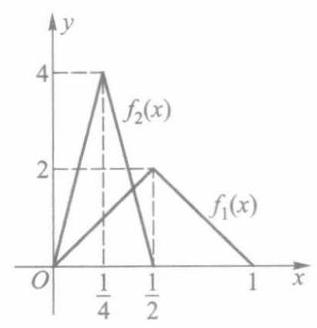
\includegraphics[width=.3\textwidth]{images/P004}
	\caption{图 $1-4$}
	\label{fig:P004}
\end{figure}

4. 确定下列初等函数的存在域:

(1) $y=\sin (\sin x);$

(2) $y=\lg (\lg x);$

(3) $y=\arcsin \left(\lg \frac{x}{10}\right);$

(4) $y=\lg \left(\arcsin \frac{x}{10}\right).$

5. 设函数
\[
f(x)= \begin{cases}
	2+x, & x \leqslant 0 \\
	2^{x}, & x>0
\end{cases}
\]
求: $(1) f(-3), f(0), f(1) ;(2) f(\Delta x)-f(0), f(-\Delta x)-f(0) \quad(\Delta x>0)$.

6. 设函数 $ f(x)=\frac{1}{1+x}, $ 求 $ f(2+x), f(2 x), f\left(x^{2}\right), f(f(x)), f\left(\frac{1}{f(x)}\right).$

7. 试问下列函数是由哪些初等函数复合而成:

(1) $y=(1+x)^{20}$;

(2) $y=\left(\arcsin x^{2}\right)^{2}$;

(3) $y=\lg \left(1+\sqrt{1+x^{2}}\right)$;

(4) $y=2^{\sin ^{2} x}$.

8. 在什么条件下, 函数
\[
y=\frac{a x+b}{c x+d}
\]

的反函数就是它本身?

9. 试作函数 $y=\arcsin (\sin x)$ 的图像.

10. 试问下列等式是否成立:

(1) $\tan (\arctan x)=x, x \in \mathbf{R}$;

(2) $ \arctan (\tan x)=x, x \neq k \pi+\frac{\pi}{2}, k=0, \pm 1, \pm 2, \cdots .$

11. 试问 $y=|x|$ 是初等函数吗?

12. 证明关于函数 $y=[x]$ 的如下不等式:

(1) 当 $x>0$ 时, $1-x<x\left[\frac{1}{x}\right] \leqslant 1$;

(2) 当 $x<0$ 时, $1 \leqslant x\left[\frac{1}{x}\right]<1-x$.

\section{具有某些特性的函数}

在本节中,我们将介绍以后常用到的几类具有某些特性的函数.

\subsection{有界函数}
\begin{definition}{有上(下) 界函数}{def:有上(下) 界函数}
	设 $f$ 为定义在 $D$ 上的函数. 若存在数 $M(L)$, 使得对每一个 $x \in D$, 有
	\[
	f(x) \leqslant M(f(x) \geqslant L)
	\]

	则称 $f$ 为 $D$ 上的有上(下) 界函数, $M(L)$ 称为 $f$ 在 $D$ 上的一个上(下)界.
\end{definition}


根据定义, $f$ 在 $D$ 上有上(下)界, 意味着值域 $f(D)$ 是一个有上(下)界的数集.又若 $M(L)$ 为 $f$ 在 $D$ 上的上 (下) 界, 则任何大于(小于) $M(L)$ 的数也是 $f$ 在 $D$ 上的上 (下)界.

\begin{definition}{有界函数}{def:有界函数}
	设 $f$ 为定义在 $D$ 上的函数.若存在正数 $M$, 使得对每一个 $x \in D$, 有
	\[
	|f(x)| \leqslant M \tag{1}
	\]
则称 $f$ 为 $D$ 上的有界函数.
\end{definition}

根据定义, $f$ 在 $D$ 上有界,意味着值域 $f(D)$ 是一个有界集. 又按定义, 不难验证: $f$ 在 $D$ 上有界的充要条件是 $f$ 在 $D$ 上既有上界又有下界. (1)式的几何意义是:若 $f$ 为 $D$ 上的有界函数,则 $f$ 的图像完全落在直线 $y=M$ 与 $y=-M$ 之间.

例如,正弦函数 $\sin x$ 和余弦函数 $\cos x$ 为 $\mathbf{R}$ 上的有界函数, 因为对每一个 $x \in \mathbf{R}$, 都 有 $|\sin x| \leqslant 1$ 和 $|\cos x| \leqslant 1$.

关于函数 $f$ 在数集 $D$ 上无上界、无下界或无界的定义,可按上述相应定义的否定 说法来叙述.例如,设 $f$ 为定义在 $D$ 上的函数,若对任何 $M$ (无论 $M$ 多大), 都存在 $x_{0} \in$ $D$, 使得 $f\left(x_{0}\right)>M$, 则称 $f$ 为 $D$ 上的无上界函数.

作为练习,读者可自行写出无下界函数与无界函数的定义.

\begin{example}
	证明 $f(x)=\frac{1}{x}$ 为 $(0,1]$ 上的无上界函数.
\end{example}


\begin{proof}
	对任何正数 $M$, 取 $(0,1]$ 上一点 $x_{0}=\frac{1}{M+1}$, 则有
	\[
	f\left(x_{0}\right)=\frac{1}{x_{0}}=M+1>M
	\]

	故按上述定义, $f$ 为 $(0,1]$ 上的无上界函数.
\end{proof}

前面已经指出, $f$ 在其定义域 $D$ 上有上界, 是指值域 $f(D)$ 为有上界的数集.于是由 确界原理,数集 $f(D)$ 有上确界.通常,我们把 $f(D)$ 的上确界记为 $\sup _{x \in D} f(x)$, 并称之为 $f$ 在 $D$ 上的上确界.类似地, 若 $f$ 在其定义域 $D$ 上有下界,则 $f$ 在 $D$ 上的下确界记为 $\inf _{x \in D} f(x).$

\begin{example}
	设 $f, g$ 为 $D$ 上的有界函数.证明:

	(i)$ \inf _{x \in D} f(x)+\inf _{x \in D} g(x) \leqslant \inf _{x \in D}\{f(x)+g(x)\} ;$

	(ii) $ \left.\sup _{x \in D} \mid f(x)+g(x)\right\} \leqslant \sup _{x \in D} f(x)+\sup _{x \in D} g(x) .$
\end{example}

\begin{proof}
	(i) 对任何 $x \in D$, 有
	\[
	\inf _{x \in D} f(x) \leqslant f(x), \inf _{x \in D} g(x) \leqslant g(x) \Rightarrow \inf _{x \in D} f(x)+\inf _{x \in D} g(x) \leqslant f(x)+g(x)
	\]

	上式表明,数 $ \inf _{x \in D} f(x)+\inf _{x \in D} g(x) $ 是函数 $ f+g $ 在 $ D $ 上的一个下界, 从而
	\[
	\inf _{x \in D} f(x)+\inf _{x \in D} g(x) \leqslant \inf _{x \in D}\{f(x)+g(x) \mid .
	\]

	(ii) 可类似地证明(略).
\end{proof}

\begin{remark}
	例 2 中的两个不等式,其严格的不等号有可能成立.例如,设
	\[
	f(x)=x, g(x)=-x, x \in[-1,1],
	\]

	则有 $\inf _{|x| \leqslant 1} f(x)=\inf _{|x| \leqslant 1} g(x)=-1, \sup _{|x| \leqslant 1} f(x)=\sup _{|x| \in \mid} g(x)=1$, 而
	\[
	\inf _{|x| \leqslant 1}\{f(x)+g(x)\}=\sup _{|x| \leqslant 1}\{f(x)+g(x)\}=0
	\]
\end{remark}


\subsection{单调函数}
\begin{definition}{单调函数}{def:单调函数}
	设 $f$ 为定义在 $D$ 上的函数.若对任何 $x_{1}, x_{2} \in D$, 当 $x_{1}<x_{2}$ 时, 总有

	(i) $f\left(x_{1}\right) \leqslant f\left(x_{2}\right)$, 则称 $f$ 为 $D$ 上的（递) 增函数, 特别当成立严格不等式 $f\left(x_{1}\right)<$ $f\left(x_{2}\right)$ 时,称 $f$ 为 $D$ 上的严格 (递) 增函数;

	(ii) $f\left(x_{1}\right) \geqslant f\left(x_{2}\right)$, 则称 $f$ 为 $D$ 上的 (递)减函数,特别当成立严格不等式 $f\left(x_{1}\right)>$ $f\left(x_{2}\right)$ 时,称 $f$ 为 $D$ 上的严格 (递) 减函数;

	增函数和减函数统称为单调函数,严格增函数和严格减函数统称为严格单调函数.
\end{definition}

\begin{example}
	函数 $y=x^{3}$ 在 $\mathbf{R}$ 上是严格增的.因为对任何 $x_{1}, x_{2} \in \mathbf{R}$, 当 $x_{1}<x_{2}$ 时, 总有
	\[
	x_{2}^{3}-x_{1}^{3}=\left(x_{2}-x_{1}\right)\left[\left(x_{2}+\frac{x_{1}}{2}\right)^{2}+\frac{3}{4} x_{1}^{2}\right]>0,
	\]

	即 $x_{1}^{3}<x_{2}^{3}$.
\end{example}

\begin{example}
	函数 $y=[x]$ 在 $\mathbf{R}$ 上是增的. 因为对任何 $x_{1}$, $x_{2} \in \mathbf{R}$, 当 $x_{1}<x_{2}$ 时显然有 $\left[x_{1}\right] \leqslant\left[x_{2}\right] .$ 但此函数在 $\mathbf{R}$ 上 不是严格增的,若取 $x_{1}=0, x_{2}=\frac{1}{2}$, 则有 $\left[x_{1}\right]=\left[x_{2}\right]=0$, 即定义中所要求的严格不等式不成立.此函数的图像如图 $1-5$ 所示.
\end{example}

\begin{figure}
	\centering
	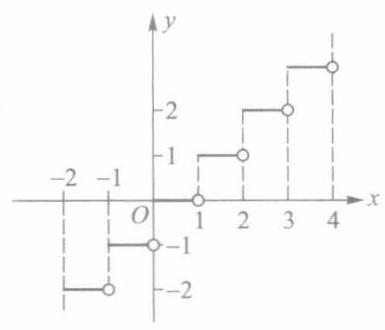
\includegraphics[width=.3\textwidth]{images/P005}
	\caption{图 $1-5$}
	\label{fig:P005}
\end{figure}

严格单调函数的图像与任一平行于 $x$ 轴的直线至多有一个交点,这一特性保证了它必定具有反函数.

\begin{theorem}{严格增(减)函数必有反函数}{the:严格增(减)函数必有反函数}
	设 $y=f(x), x \in D$ 为严格增(减) 函数, 则 $f$ 必有反函数 $f^{-1}$, 且 $f^{-1}$ 在其定 义域 $f(D)$ 上也是严格增( 减) 函数.
\end{theorem}

\begin{proof}
	设 $f$ 在 $D$ 上严格增.对任一 $y \in f(D)$, 有 $x \in D$ 使 $f(x)=y .$ 下面证明这样的 $x$ 只 能有一个.事实上,对于 $D$ 中任一 $x_{1} \neq x$, 由 $f$ 在 $D$ 上的严格增性, 当 $x_{1}<x$ 时, $f\left(x_{1}\right)<y$, 当 $x_{1}>x$ 时, 有 $f\left(x_{1}\right)>y$, 总之 $f\left(x_{1}\right) \neq y$. 这就说明, 对每一个 $y \in f(D)$, 都只存在唯一的一个$x \in D$, 使得 $f(x)=y$, 从而函数 $f$ 存在反函数 $x=f^{-1}(y), y \in f(D)$.

	现证 $f^{-1}$ 也是严格增的.任取 $y_{1}, y_{2} \in f(D), y_{1}<y_{2} .$ 设 $x_{1}=f^{-1}\left(y_{1}\right), x_{2}=f^{-1}\left(y_{2}\right)$, 则 $y_{1}=f\left(x_{1}\right), y_{2}=f\left(x_{2}\right)$. 由 $y_{1}<y_{2}$ 及 $f$ 的严格增性, 显然有 $x_{1}<x_{2}$, 即 $f^{-1}\left(y_{1}\right)<f^{-1}\left(y_{2}\right)$. 所以反函数 $f^{-1}$ 是严格增的.
\end{proof}

\begin{example}
	函数 $y=x^{2}$ 在 $[0,+\infty)$ 上是严格增的, 由 $\S 3$ 例 1 可知, 其值域为 $[0,+\infty)$, 故有反函数 $y=\sqrt{x}, x \in[0,+\infty)$; 函数 $y=x^{2}$ 在 $(-\infty, 0)$ 是严格减的, 有反函数 $y=-\sqrt{x}$, $x \in(0,+\infty)$.但 $y=x^{2}$ 在整个定义域 $\mathbf{R}$ 上不是单调的, 也不存在反函数.
\end{example}


上节中我们给出了实指数幕的定义,从而将指数函数
\[
y=a^{x}(a>0, a \neq 1)
\]
的定义域拓广到整个实数集 $\mathbf{R} .$ 下面证明指数函数在 $\mathbf{R}$ 上的严格单调性.

\begin{example}
	证明: $y=a^{x}$ 当 $a>1$ 时在 $\mathbf{R}$ 上严格递增, 当 $0<a<1$ 时在 $\mathbf{R}$ 上严格递减.
\end{example}

\begin{proof}
	设 $a>1 .$ 给定 $x_{1}, x_{2} \in \mathbf{R}, x_{1}<x_{2}$. 由有理数集的稠密性, 可取到有理数 $r_{1}, r_{2}$, 使 $x_{1}<r_{1}<r_{2}<x_{2}$ (参见 $\S 1$ 例 1 ), 故有
	\[
	\begin{aligned}
		a^{x_{1}} &=\sup _{i \leqslant x_{1}}\left\{a^{r} \mid r \text { 为有理数 }\right\} \leqslant a^{r_{1}} \\
		&<a^{r_{2}} \leqslant \sup _{i \leqslant x_{2}}\left\{a^{r} \mid r \text { 为有理数 }\right\}=a^{x_{2}},
	\end{aligned}
	\]

	这就证明了 $a^{x}$ 当 $a>1$ 时在 $\mathbf{R}$ 上严格递增.

	类似地可证 $a^{x}$ 当 $0<a<1$ 时在 $\mathbf{R}$ 上严格递减.
\end{proof}

\begin{remark}
	因为 $y=a^{x}(a>0, a \neq 1)$ 的值域为 $(0,+\infty)$, 所以由例 6 及定理 $1.2$ 还可得出结论: 对数函数 $y=\log _{a} x$ 当 $a>1$ 时在 $(0,+\infty)$ 上严格递增, 当 $0<a<1$ 时在 $(0,+\infty)$ 上严格递减.另外,在第四章中将证明关于实指数幂的一个基本性质 $\left(a^{\alpha}\right)^{\beta}=a^{\alpha \beta}$ (定理 4.10 ), 从而相应地有
	\[
	\log _{a} x^{\alpha}=\alpha \log _{a} x\left(a>0, a \neq 1, x \in \mathbf{R}^{+}, \alpha \in \mathbf{R}\right) \tag{2}
	\]
\end{remark}


\subsection{奇函数和偶函数}
\begin{definition}{奇（偶)函数}{def:奇（偶)函数}
	设 $D$ 为对称于原点的数集, $f$ 为定义在 $D$ 上的函数.若对每一个 $x \in D$, 有
	\[
	f(-x)=-f(x) \quad(f(-x)=f(x)),
	\]

	则称 $f$ 为 $D$ 上的奇(偶)函数.
\end{definition}

从函数图形上看,奇函数的图像关于原点对称,偶函数的图像则关于 $y$ 轴对称.

例如, 正弦函数 $y=\sin x$ 和正切函数 $y=\tan x$ 是奇函数, 余弦函数 $y=\cos x$ 是偶函 数, 符号函数 $y=\operatorname{sgn} x$ 是奇函数(见图 $1-1$ ). 而函数 $f(x)=\sin x+\cos x$ 既不是奇函数, 也不是偶函数, 因若取 $x_{0}=\frac{\pi}{4}$, 则 $f\left(x_{0}\right)=\sqrt{2}, f\left(-x_{0}\right)=0$, 显然既不成立 $f\left(-x_{0}\right)=-f\left(x_{0}\right)$, 也不成立 $f\left(-x_{0}\right)=f\left(x_{0}\right)$.

\subsection{周期函数}

设 $f$ 为定义在数集 $D$ 上的函数.若存在 $\sigma>0$, 使得对一切 $x \in D, x \pm \sigma \in D$, 有 $f(x \pm \sigma)=f(x)$, 则称 $f$ 为\textbf{周期函数}, $\sigma$ 称为 $f$ 的一个\textbf{周期}. 显然, 若 $\sigma$ 为 $f$ 的周期, 则 $n \sigma$($n$ 为正整数）也是 $f$ 的周期.若在周期函数 $f$ 的所有周期中有一个最小的周期,则称此最小周期为 $f$ 的\textbf{基本周期}, 或简称\textbf{周期}.

例如, $\sin x$ 的周期为 $2 \pi, \tan x$ 的周期为 $\pi$. 函数
\[
f(x)=x-[x], x \in \mathbf{R}
\]
的周期为 1 (见图 1-6 ).常量函数 $f(x)=c$ 是以任何正数为周期的周期函数,但不存在基本周期.

\begin{figure}
	\centering
	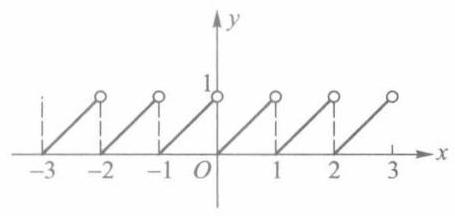
\includegraphics[width=.3\textwidth]{images/P006}
	\caption{图 $1-6$}
	\label{fig:P006}
\end{figure}

\subsection{习题1.4}
1. 证明 $f(x)=\frac{x}{x^{2}+1}$ 是 $\mathbf{R}$ 上的有界函数.

2. (1) 叙述无界函数的定义;

(2) 证明 $f(x)=\frac{1}{x^{2}}$ 为 $(0,1)$ 上的无界函数;

(3) 举出函数 $f$ 的例子,使 $f$ 为闭区间 $[0,1]$ 上的无界函数.

3. 证明下列函数在指定区间上的单调性:

(1)$ y=3 x-1 $ 在 $(-\infty,+\infty) $ 上严格递增;

(2) $y=\sin x$ 在 $\left[-\frac{\pi}{2}, \frac{\pi}{2}\right]$ 上严格递增;

(3) $y=\cos x$ 在 $[0, \pi]$ 上严格递减.

4. 判别下列函数的奇偶性:

(1) $ f(x)=\frac{1}{2} x^{4}+x^{2}-1 ; $

(2) $ f(x)=x+\sin x_{i};$

(3) $f(x)=x^{2} \mathrm{e}^{-x^{2}};$

(4) $ f(x)=\lg \left(x+\sqrt{1+x^{2}}\right) .$


5. 求下列函数的周期：

(1) $ \cos ^{2} x_{i} ;$

(2) $ \tan 3 x_{i} ;$

(3) $ \cos \frac{x}{2}+2 \sin \frac{x}{3} .$


6. 设函数 $f$ 定义在 $[-a, a]$ 上, 证明：

(1) $F(x)=f(x)+f(-x), x \in[-a, a]$ 为偶函数

(2) $G(x)=f(x)-f(-x), x \in[-a, a]$ 为奇函数;

(3) $f$ 可表示为某个奇函数与某个偶函数之和.

7. 由三角函数的两角和(差)公式
\[
\begin{aligned}
	&\sin (\alpha \pm \beta)=\sin \alpha \cos \beta \pm \sin \beta \cos \alpha \\
	&\cos (\alpha+\beta)=\cos \alpha \cos \beta \mp \sin \alpha \sin \beta
\end{aligned}
\]

推出:

(1) 和差化积公式
\[
\begin{aligned}
	&\sin \alpha+\sin \beta=2 \sin \frac{\alpha+\beta}{2} \cos \frac{\alpha-\beta}{2} \\
	&\sin \alpha-\sin \beta=2 \sin \frac{\alpha-\beta}{2} \cos \frac{\alpha+\beta}{2} \\
	&\cos \alpha+\cos \beta=2 \cos \frac{\alpha+\beta}{2} \cos \frac{\alpha-\beta}{2} \\
	&\cos \alpha-\cos \beta=-2 \sin \frac{\alpha+\beta}{2} \sin \frac{\alpha-\beta}{2}
\end{aligned}
\]

(2) 积化和差公式
\[
\begin{aligned}
	&\sin \alpha \sin \beta=\frac{1}{2}[\cos (\alpha-\beta)-\cos (\alpha+\beta)] \\
	&\sin \alpha \cos \beta=\frac{1}{2}[\sin (\alpha+\beta)+\sin (\alpha-\beta)] \\
	&\cos \alpha \cos \beta=\frac{1}{2}[\cos (\alpha+\beta)+\cos (\alpha-\beta)]
\end{aligned}
\]

8. 设 $f, g$ 为定义在 $D$ 上的有界函数,满足
\[
f(x) \leqslant g(x), x \in D
\]

证明 :(1) $\sup _{x \in D} f(x) \leqslant \sup _{x \in D} g(x) ; $

(2) $ \inf _{x \in D} f(x) \leqslant \inf _{x \in D} g(x) .$

9. 设 $ f $ 为定义在 $ D ${ 上的有界函数, 证明：

(1) $ \sup _{x \in D}\{-f(x)\}=\underset{x \in D}{-\inf f(x)} ;$

(2) $ \inf _{x \in D}\{-f(x)\}=\underset{x \in D}{\sup } f(x) .$

10. 证明 : $ \tan x $ 在 $\left(-\frac{\pi}{2}, \frac{\pi}{2}\right) $ 上无界,而在任一闭区间 $[a, b] \subset\left(-\frac{\pi}{2}, \frac{\pi}{2}\right) $ 上有界.

11. 讨论狄利克雷函数
\[
D(x)=\left\{\begin{array}{l}
	1, \text { 当 } x \text { 为有理数, } \\
	0, \text { 当 } x \text { 为无理数 }
\end{array}\right.
\]

的有界性、单调性与周期性.

12. 证明 : $f(x)=x+\sin x $ 在 $ \mathbf{R} $ 上严格增.

13. 设定义在 $[a,+\infty) $ 上的函数 $ f $ 在任何闭区间 $[a, b] $ 上有界. 定义 $[a,+\infty) $ 上的函数：
\[
m(x)=\inf _{a \leqslant y \leqslant x} f(y), \quad M(x)=\sup _{a \leq y \in x} f(y) \text {. }
\]

试讨论 $m(x)$ 与 $M(x)$ 的图像, 其中

(1) $ f(x)=\cos x, x \in[0,+\infty) ; $

(2) $ f(x)=x^{2}, x \in[-1,+\infty) .$

\section{第一章总练习题}

1. 设 $a, b \in \mathbf{R}$, 证明：

(1) $ \max \{a, b\}=\frac{1}{2}(a+b+|a-b|) ;$

(2) $\min \{a, b\}=\frac{1}{2}(a+b-|a-b|).$

2. 设 $f$ 和 $g$ 都是 $D$ 上的初等函数.定义
\[
M(x)=\max \mid f(x), g(x)\}, m(x)=\min \{f(x), g(x)\}, x \in D
\]

试问 $M(x)$ 和 $m(x)$ 是否为初等函数?

3. 设函数 $ f(x)=\frac{1-x}{1+x} $, 求：
\[
f(-x), f(x+1), f(x)+1, f\left(\frac{1}{x}\right), \frac{1}{f(x)}, f\left(x^{2}\right), f(f(x))
\]

4. 已知 $f\left(\frac{1}{x}\right)=x+\sqrt{1+x^{2}}$, 求 $f(x)$.

5. 利用函数 $y=[x]$ 求解:

(1) 某系各班级推选学生代表,每 5 人推选 1 名代表,余额满 3 人可增选 1 名.写出可推选代表数 $y$ 与班级学生数 $x$ 之间的函数关系(假设每班学生数为 $30 \sim 50$ 人);

(2) 正数 $x$ 经四舍五人后得整数 $y$,写出 $y$ 与 $x$ 之间的函数关系.

6. 已知函数 $y=f(x)$ 的图像,试作下列各函数的图像:

(1) $ y=-f(x) ;$

(2) $y=f(-x) ;$

(3) $y=-f(-x) ;$

(4) $y=|f(x)| ; $

(5) $y=\operatorname{sgn} f(x) ;$

(6) $ y=\frac{1}{2}[|f(x)|+f(x)] ;$

(7) $y=\frac{1}{2}[|f(x)|-f(x)]$.

7. 已知函数 $f$ 和 $g$ 的图像,试作下列函数的图像:

(1) $\varphi(x)=\max \{f(x), g(x)\} ; $

(2) $\psi(x)=\min |f(x), g(x)|.$

8. 设 $f, g$ 和 $h$ 为增函数,满足
\[
f(x) \leqslant g(x) \leqslant h(x), x \in \mathbf{R} .
\]

证明: $f(f(x)) \leqslant g(g(x)) \leqslant h(h(x))$.

9. 设 $f$ 和 $g$ 为区间 $(a, b)$ 上的增函数,证明第 7 题中定义的函数 $\varphi(x)$ 和 $\psi(x)$ 也都是 $(a, b)$ 上的增函数.

10. 设 $f$ 为 $[-a, a]$ 上的奇 $($ 偶) 函数.证明:若 $f$ 在 $[0, a]$ 上增,则 $f$ 在 $[-a, 0]$ 上增 (减).

11. 证明:

(1) 两个奇函数之和为奇函数,其积为偶函数;

(2) 两个偶函数之和与积都为偶函数;

(3) 奇函数与偶函数之积为奇函数.

12. 设 $f, g$ 为 $D$ 上的有界函数.证明：

(1) $ \inf _{x \in D}|f(x)+g(x)| \leqslant \inf _{x \in D} f(x)+\sup _{x \in D} g(x) ;$

(2) $\left.\sup _{x \in D} f(x)+\inf _{x \in D} g(x) \leqslant \sup _{x \in D} \mid f(x)+g(x)\right\}$.


13. 设 $f, g$ 为 $D$ 上的非负有界函数.证明:

(1) $ \left.\inf _{x \in D} f(x) \cdot \inf _{x \in D} g(x) \leqslant \inf _{x \in D} \mid f(x) g(x)\right\}$



14. 将定义在 $(0,+\infty)$ 上的函数 $f$ 延拓到 $\mathbf{R}$ 上,使延拓后的函数为 (i) 奇函数; (ii) 偶函数.设

(1) $f(x)=\sin x+1$;

(2) $f(x)= \begin{cases}
	1-\sqrt{1-x^{2}}, & 0<x \leqslant 1 \\
	x^{3}, & x>1
\end{cases}$

15. 设 $f$ 为定义在 $\mathbf{R}$ 上以 $h$ 为周期的函数, $a$ 为实数. 证明:若 $f$ 在 $[a, a+h]$ 上有界,则 $f$ 在 $\mathbf{R}$ 上有界.

16. 设 $f$ 在区间 $I$ 上有界. 记
\[
M=\sup _{x \in !} f(x), \quad m=\inf _{x \in I} f(x)
\]

证明
\[
\sup _{x^{\prime}, x^{\prime \prime} \in \mid}\left|f\left(x^{\prime}\right)-f\left(x^{\prime \prime}\right)\right|=M-m
\]

17. 设
\[
f(x)=\left\{\begin{array}{l}
	q, \quad \text { 当 } x=\frac{p}{q}\left(p, q \in \mathbf{N}_{+}, \frac{p}{q} \text { 为既约真分数 }, 0<p<q\right), \\
	0, x \text { 为 }(0,1) \text { 中的无理数. }
\end{array}\right.
\]

证明:对任意 $x_{0} \in(0,1)$, 任意正数 $\delta,\left(x_{0}-\delta, x_{0}+\delta\right) \subset(0,1)$, 有 $f(x)$ 在 $\left(x_{0}-\delta, x_{0}+\delta\right)$ 上无界.

18. 设 $a>0, m, n, p$ 为正整数,规定 $a^{\frac{m}{n}}=\left(a^{\frac{1}{n}}\right)^{m}$. 证明 $: a^{\frac{p m}{m^{m}}}=\left(a^{\frac{1}{p^{n}}}\right)^{p m}=a^{\frac{m}{n}}$.


\section{第一章综合自测题}

